% This file should be replaced with your file with an thesis content.
%=========================================================================
% Authors: Michal Bidlo, Bohuslav Křena, Jaroslav Dytrych, Petr Veigend and Adam Herout 2019

% For compilation piecewise (see projekt.tex), it is necessary to uncomment it and change
% \documentclass[../projekt.tex]{subfiles}
% \begin{document}


\chapter{Introduction}

Although more than 30 years have passed since the invention of the web back in 1989 \cite{WWWProposal}, it is still an integral part of our lives, possibly more than ever before. People worldwide use the web daily to work, learn, consume content and connect with others. Every day our smartphones, tablets, laptops, or even smartwatches and fridges connect to the web.

This diverse ecosystem of devices created a need to identify users who use them uniquely. The ability to uniquely identify a user on a single device or across multiple devices allows applications to personalize the content they provide or improve their security.
One of the methods of user identification is browser fingerprinting, the collection of data from the browser to create a fingerprint of the device. Just as a person's fingerprint can uniquely identify that specific person, given that we have enough data, we can uniquely identify a device and its user and act on this information.

However, gathering this kind of data can be considered a violation of privacy \cite{WP224Fingerprinting}, which is the primary motivation behind creating privacy-first browsers and browser extensions to fight against fingerprinting. One of the browser extensions set on improving privacy is JShelter\footnote{JShelter is an anti-malware browser extension to mitigate potential threats from JavaScript, including fingerprinting \cite{JShelterHome} (Available at \url{https://jshelter.org/}).} which focuses on preventing active fingerprinting.

Active fingerprinting is a method of obtaining a fingerprint, typically by running JavaScript code to collect data from browser APIs \cite{FingerprintingSurvey}. The other variant is passive fingerprinting, in which the data is collected solely from network traffic, for example, HTTP headers.

This work aims to design and implement a browser extension to prevent the collection of passive fingerprints by altering data in HTTP requests and explore possibilities of integrating this protection into JShelter. It is important to note that the altered data must be consistent with the data obtainable through active fingerprinting methods. Otherwise, the fingerprinting application could recognize an attempt to mitigate the effects of fingerprinting.

Fingerprinting is an ever-evolving field. Chapter \ref{Chapter:BrowserFingerprinting} describes its nature, history, and different approaches to collecting a fingerprint. The last two sections of chapter \ref{Chapter:BrowserFingerprinting} provide an outlook on threats and opportunities fingerprinting brings to the table because, as we know, nothing is purely black and white.

As this work explores the capabilities of mitigating fingerprinting with the help of browser extensions, the following chapter \ref{Chapter:Extensions} gives the reader an insight into the inner working of extensions.

Finally, the last chapter \ref{Chapter:Design} proposes a design of passive fingerprinting protection that works consistently with active solutions to keep user-observable side effects to a minimum.

\section{Definitions}

\begin{itemize}
	\item \textbf{Fingerprint}: A collection of device-specific characteristics gathered for the purpose of identification.
	\item \textbf{Fingerprinting}: The process of collecting the device information (data) to compute a fingerprint. Terms fingerprinting, device fingerprinting, and browser fingerprinting will be used interchangeably in the following chapters.
	\item \textbf{Fingerprinter}: An application performing fingerprinting, typically on a third-party remote server.
\end{itemize}

% -------------------------------------------------------------------- %

\chapter{Web browsers}
% TODO: Chapter description. The part below is copied from the old chapter "web extensions".

In this chapter, the first section, \ref{Section:WebExtensionsAPI}, describes the WebExtensions API exposed by a browser to give extensions more capabilities. Recently, significant changes to the ecosystem of extensions were announced with the introduction of Manifest V3, described in section \ref{Section:ManifestV3}. The last section, \ref{Section:JShelter}, is dedicated to the JShelter extension on which this work builds.

\section{History of web browsers}

Web browsers have come a long way since the early days of the World Wide Web. From their humble beginnings as basic applications for viewing text-only web pages, modern browsers have evolved into the powerful tools we know today. Following paragraphs outline the evolution of browsers, highlighting a few of the most significant features added over the years.

The first browser, named WorldWideWeb\footnote{\url{https://worldwideweb.cern.ch}}, was created at CERN by Tim Berners-Lee only a year after he published the first World Wide Web proposal \cite{WWWProposal}. The very early browser aimed to demonstrate how the user-facing layer of the WWW (browsers) could work in the future. The browser was only available on the NeXTSTEP\footnote{\url{https://en.wikipedia.org/wiki/NeXTSTEP}} operating system and had limited features.

One of the earliest features added to browsers was support for images. The Mosaic browser\footnote{\url{https://en.wikipedia.org/wiki/Mosaic_(web_browser)}}, released in 1993, was the first to allow users to view images on the web, followed by support for tables, which allowed for more complex web page layouts.

As the web gained popularity, developers needed a way to make web pages more interactive and dynamic. The birth of JavaScript programming language addressed this need. JavaScript was first introduced in 1995\footnote{\url{https://en.wikipedia.org/wiki/Netscape_Navigator_2}} by Netscape Communications Corporation to add interactivity to static HTML pages. Since then, it has become one of the world's most widely used programming languages, with a vast ecosystem of libraries and frameworks\footnote{\url{https://www.npmjs.com/}}.

Nowadays, web browsers expose a variety of JavaScript APIs that allow web developers to interact with the browser and its underlying components, such as the operating system or even the hardware. While it is true that these APIs gave the developers much-needed possibilities, they come at the cost of compromised privacy, described in detail in the following chapters.

\section{JavaScript}

In its original form, JavaScript is a client-side language executed in the user's web browser rather than on a web server \cite{JSDefinitiveGuide}. It allows applications to respond to user actions in real time without making a round trip to the server. However, the rise of popularity and the fact that JavaScript is a relatively developer-friendly language meant that, eventually, runtimes that allowed running JavaScript outside the browser emerged. The most popular JavaScript runtimes include Node.js\footnote{\url{https://nodejs.org/}}, Deno\footnote{\url{https://deno.land/}}, or Bun\footnote{\url{https://bun.sh/}}.

\subsection{ECMAScript}

As the web was rapidly gaining popularity, developers started using JavaScript to create dynamic and interactive web pages. However, there was no standardization for the language, meaning different browsers implemented JavaScript differently. This made it difficult for developers to create web applications that worked consistently across different platforms and browsers \cite{JSDefinitiveGuide}.

In 1996, Netscape Communications Corporation, the company behind the Netscape Navigator web browser, submitted JavaScript to ECMA International\footnote{\url{https://www.ecma-international.org/}}. This standards organization develops and maintains standards for several technologies, including programming languages. The goal was to create a standardized language version that could be implemented across different platforms and browsers.

ECMA International established a committee to develop a standardized scripting language, which was initially called ECMA-262. The standard's first version, ECMAScript 1, was released in June 1997. Since then, ECMAScript has undergone several revisions, the latest being ECMAScript 2022. Each standard version adds new features and capabilities to the language while maintaining backward compatibility with previous versions \cite{JSDefinitiveGuide}.

Although ECMAScript is technically the correct name for the language, JavaScript is used in the following chapters as the industry uses this name predominantly.

\subsection{Web APIs}

Web applications can use JavaScript Web APIs to interact with various web browser features and functionality. The number of available APIs depends on the browser. For example, at the time of the writing, Firefox had more than 100 APIs\footnote{\url{https://developer.mozilla.org/en-US/docs/Web/API}}, with more APIs still being added. Here is a short selection of Web APIs important to the topic of this thesis \cite{SecurityWebDevs, SchauerDP}:

\begin{itemize}
	\item \textbf{Canvas API}: Provides a way to dynamically create and manipulate graphics and animations in a web page using JavaScript.
	\item \textbf{Navigator}: Provides information about the web browser or user agent in which the code runs.
	\item \textbf{Web Audio API}: Provides advanced audio processing and synthesis capabilities, allowing developers to create interactive audio experiences on the web.
	\item \textbf{WebGL}: Allows for creating and rendering interactive 3D and 2D graphics within a web browser using the computer's graphics hardware capabilities.
\end{itemize}

All the APIs listed above are commonly used in fingerprinting to identify devices and their users uniquely \cite{FingerprintingSurvey}. Fingerprinting, the main focus of this thesis, is described more in-depth in the following chapter.

\section{HTTP}

HTTP (Hypertext Transfer Protocol) is a request-response protocol that allows web browsers to request resources from web servers and to receive responses that include the requested resources \cite{MasteringNodeJS}.

When a user types a URL into a web browser's address bar, the browser sends an HTTP request to the server hosting the resource. This request typically contains information such as the request's method, the URL of the requested resource, and any HTTP headers or other metadata associated with the request. The server then resolves the request and sends a response containing the response status code and body, among other things.

Web applications can also ask the browser to send HTTP requests on their behalf with the help of XMLHttpRequest (XHR)\footnote{\url{https://developer.mozilla.org/en-US/docs/Web/API/XMLHttpRequest}} or Fetch API\footnote{\url{https://developer.mozilla.org/en-US/docs/Web/API/Fetch_API}} APIs. Web applications commonly transfer only minimal HTML and JavaScript with the first request to improve performance. Once loaded, this skeleton can load additional resources if needed.

\subsection{Headers}

The client and the server use HTTP headers\footnote{\url{https://developer.mozilla.org/en-US/docs/Web/HTTP/Headers}} to transfer additional information with the HTTP request or response. Headers consist of a case-insensitive name and a value separated by a colon (\uv{:}). HTTP defines standardized headers for content negotiation, authentication, or passing additional context \cite{RFC9110}. The protocol also allows the use of entirely custom headers.

When an application sends a request, the browser automatically includes default headers. Web applications can add additional headers or overwrite the default ones.

\section{Browser extensions}

Browser extensions, or add-ons, can modify and enhance the capability of a browser \cite{MDNWebExtensions}. Users install extensions for various reasons, such as to increase security or productivity, remove ads, or modify the browser UI to their liking. Each browser implements extensions slightly differently, but to a large extent, most browsers follow the WebExtensions API standard.

This section describes the WebExtensions API standard mentioned before and the recently introduced Manifest V3, which significantly affects the ecosystem of browser extensions.

\label{Chapter:Extensions}

\subsection{WebExtensions API}
\label{Section:WebExtensionsAPI}

WebExtensions API, first introduced by Google in chromium-based browsers, is a set of special-purpose APIs the browser provides to installed extensions. Firefox\footnote{\url{https://developer.mozilla.org/en-US/docs/Mozilla/Add-ons/WebExtensions}}, Safari\footnote{\url{https://developer.apple.com/documentation/safariservices/safari_web_extensions}}, and Opera\footnote{\url{https://dev.opera.com/extensions/apis}} have become widely compatible with the WebExtensions API, making it the standard across all major web browsers. This broad adoption allowed developers to create cross-browser extensions with minor changes to the original codebase.

WebExtensions API provides a wide range of functionality for building browser extensions, including access to browser tabs and windows, manipulating web pages and user settings, and interacting with other extensions and websites \cite{ChromeWebExtensions}.

WebExtension API differs from the standard JavaScript Web APIs described in the previous section. Applications use the standard Web APIs to interact with the content and functionality of a web page. In contrast, extensions use the WebExtensions APIs to interact with the browser itself. Some of the interfaces provided by the WebExtensions API are \cite{ChromeWebExtensions}:

\begin{itemize}
	\item \textbf{Cookies API}: Allows to query and modify cookies. Extensions can also configure a callback function browser calls whenever a particular cookie changes.
	\item \textbf{DeclarativeNetRequest API}: Allows to block or modify network requests by specifying declarative rules. This API allows extensions to modify requests without giving them direct access to their content.
	\item \textbf{History API}: Allows interaction with the browser's record of previously visited pages. Extensions can add, remove, and query for URLs in the browser's history.
	\item \textbf{Tabs API}: Allows interaction with the browser's tab system. Extensions can create new, modify, or rearrange existing tabs.
\end{itemize}

The WebExtensions API is easy to use and provides consistent interfaces and functionality across different browsers. Lately, a push for increased security and privacy rules for extensions resulted in Manifest V3, described more in-depth in the following section.

\subsection{Browser extension architecture}

Extensions, in their essence, are lightweight software modules that are running in the browser. Every extension acts independently from the browser and all other installed extensions. Like regular web pages, extensions are developed using HTML, CSS, and JavaScript.

A typical architecture of a browser extension consists of several components that work together to achieve the desired functionality. These components include \cite{ChromeWebExtensions}:

\begin{itemize}
	\item \textbf{Manifest file}: A required JSON file in the root of the extension source directory that contains metadata about the extension, such as its name, version, description, and permissions. It also defines the various components of the extension and their roles.
	\item \textbf{Service workers (background scripts)}: JavaScript files that run in the background and handle the core logic of the extension. They manage persistent states, listen for browser events, and interact with Web APIs.
	\item \textbf{Content scripts}: JavaScript files that run in the context of a web page and have access to the DOM of that page. They enable the extension to read or modify the content of web pages and interact with user actions. Content scripts run in an isolated environment, limiting their access to the same-origin policy of the web page.
	\item \textbf{Popups}: An optional user interface that provides a quick and easy way for users to interact with the extension. It usually appears when a user clicks on the extension's icon in the browser toolbar. Popups are transient and close when they lose focus.
	\item \textbf{Options}: An optional user interface that allows users to configure the settings and preferences of the extension. The options page is accessible through the browser's extension management interface.
\end{itemize}

In summary, the typical architecture of a browser extension involves a Manifest file that points to other files this extension defines.

\subsubsection{Manifest file}

The Manifest file is the only file that must be present in every extension. The file must have the name `manifest.json` and be in the extension's root directory.

Out of all the configuration fields the Manifest file supports, only three of these fields are mandatory, according to the Manifest file format documentation\footnote{\url{https://developer.chrome.com/docs/extensions/mv3/manifest/}}:

\begin{itemize}
	\item \textbf{manifest\_version}: An integer value specifying the version of the Manifest file. Since June 2022, the only allowed value by the Chrome Web Store\footnote{{\url{https://chrome.google.com/webstore/category/extensions}}} has been \uv{3} for all newly added extensions. The January 2024 deadline, when the Chrome Web Store stops accepting updates to existing Manifest V2 extensions, has been postponed, meaning there is no official date for the end of life of Manifest V2.
	\item \textbf{name}: A plain text string identifying the extension in the Chrome Web Store and the Browser UI.
	\item \textbf{version}: A version string consisting of one to three integers separated by dots. Version numbers must be strictly incremental as the browser uses them to decide whether an extension should be updated.
\end{itemize}

Apart from the three mandatory fields, the Manifest file supports a wide range of other configuration options, including:

\begin{itemize}
	\item \textbf{action}: An object defining the extension's button in the browser's toolbar. Clicking on this button opens the popup if the extension defines it. Otherwise, clicking this button will dispatch an event to the extension's background scripts.
	\item \textbf{background}: Used to include one or more background scripts. For newer Manifest V3 extensions, this configuration field is used to include service worker scripts. Extension service workers do not run on the main thread, meaning they do not interfere with extension content.
	\item \textbf{permissions}: An array of string keys specifying the granular permissions the extension requires. The browser informs the user what permissions the extension requires during installation.
\end{itemize}

In January 2022, the Chrome Web Store began the long-awaited transition to the new version of the Manifest file, Manifest V3. The Manifest V3 represents one of the most significant shifts in the extensions platform since its launch \cite{ChromeWebExtensions}. According to the team behind the Chrome browser, it is an answer to raising concerns about privacy, security, and performance of browser extensions. The most notable changes compared to its predecessor Manifest V2 are \cite{ChromeWebExtensions}:

\begin{itemize}
	\item \textbf{Service workers}: Manifest V3 replaces background pages\footnote{Manifest V2 extensions used background pages to run a single persistent script to manage tasks, or a state of the extension \cite{ChromeManifestV2}.} with extension service workers, similar to traditional web service workers.
	\item \textbf{Network request modification}: In the outgoing Manifest V2, extensions could intercept and modify requests procedurally. In contrast, in the Manifest V3, extensions have to define rules and ask the browser engine to modify requests on their behalf. The primary motivation behind this change was privacy, as extensions could previously access requests with little or no limitations.
	\item \textbf{Support for Promises}: The Chrome team added Promise support to some WebExtensions APIs so that extension developers can use modern JavaScript features such as promise chains or async/await patterns.
\end{itemize}

Although welcomed from a privacy-concerned standpoint, these changes made it more difficult for developers to create extensions to protect from fingerprinting, mainly because of the network request modification differences.

\bigbreak

\begin{lstlisting}[language={JSON},caption={An example of a declarative rule which modifies selected response headers \cite{ChromeWebExtensions}.}, label={Listing:ManifestV3RuleExample}]
[
  {
    "id": 10,
    "priority": 2,
    "action": {
      "type": "modifyHeaders",
      "responseHeaders": [
        {
          "header": "h1",
          "operation": "remove"
        },
        {
          "header": "h2",
          "operation": "set",
          "value": "v2"
        },
        {
          "header": "h3",
          "operation": "append",
          "value": "v3"
        }
      ]
    },
    "condition": {
      "urlFilter": "headers.com/123",
      "resourceTypes": ["main_frame"]
    }
  }
]
\end{lstlisting}

\medbreak

Listing \ref{Listing:ManifestV3RuleExample} shows an example of the new declarative rule syntax. The rule defined above modifies request headers, specifically removing a header named \texttt{h1}, changing the value of \texttt{h2}, and adding a new header, \texttt{h3}.

At the time of the writing, Manifest V2 extensions are transitioning to Manifest V3. Although no official date is set\footnote{\url{https://developer.chrome.com/docs/extensions/migrating/mv2-sunset/}}, the Chrome Web Store will eventually stop accepting updates to old Manifest V2 extensions. For this reason and to avoid confusion, this thesis will only consider Manifest V3 in the following chapters.

\subsubsection{Service workers}

Extension service workers represent a significant update in how browser extensions handle background tasks, focusing on enhancing security, privacy, and performance. Replacing the previously used background scripts, service workers offer more efficient resource management, better offline capabilities, and improved security features for browser extensions. This shift aligns with the ongoing evolution of web technologies\footnote{{\url{https://developer.chrome.com/docs/extensions/mv3/intro/platform-vision/}}} and the need for a more secure and reliable foundation for extension development.

Service workers are event-driven, meaning they only run when needed, unlike persistent background scripts \cite{ChromeWebExtensions}. This reduction in resource consumption improves the overall performance of the browser. Additionally, service workers can cache resources and intercept network requests, enabling them to work efficiently even when the user is offline. This feature can enhance the responsiveness and reliability of extensions, even under poor network conditions.

Enhanced security is another significant benefit of service workers in Manifest V3 extensions. Running in a separate thread from the main browser process and having a limited scope, service workers help reduce the attack surface of extensions. With a more restrictive API surface compared to background pages, the risks associated with potential security vulnerabilities are minimized. Introducing service workers in Manifest V3 offers a more secure, efficient, and reliable foundation for developing browser extensions.

Service workers cannot access the DOM API as they are running in a separate thread. Extensions that want to modify the DOM must do so in an alternative API, such as the Offscreen API\footnote{\url{https://developer.chrome.com/docs/extensions/reference/offscreen/}}.

\subsubsection{Content scripts}

Extension content scripts are an essential component of browser extensions that enable interaction with web pages displayed in the browser. They provide a means for the extension to read or modify the content of a web page, access the DOM, and manipulate CSS styles. Content scripts bridge the gap between the isolated extension environment and the web pages it aims to enhance, enabling a wide range of functionality, from modifying the appearance of a website to implementing custom features.

Content scripts run in the context of the web pages they are injected into but maintain a separate JavaScript environment \cite{ChromeWebExtensions}. This separation ensures that content scripts do not directly interact with the JavaScript running on the web page, preventing potential conflicts or security issues. Despite the separation, content scripts can still communicate with the web page's JavaScript using custom events or other messaging mechanisms\footnote{\url{https://developer.chrome.com/docs/extensions/mv3/content_scripts/\#host-page-communication}}.

To use content scripts in a browser extension, developers must declare them in the extension's manifest file, specifying which scripts to inject and the conditions under which they should be injected, such as the URL patterns of the target web pages. Once configured, the browser extension can seamlessly augment or modify web pages, providing users with customized experiences and extended functionality tailored to their needs.

\subsubsection{Popups}

Extension popups are standalone HTML documents associated with the extension's button in the browser toolbar \cite{ChromeWebExtensions}. When a user clicks the button, the browser will show a popup. Popups are closed when a user either outside the popup or again on the extension's toolbar button.

Like standard web pages, the popup's HTML document can import external CSS and JavaScript files. Unlike standard web pages, however, the popup can access the WebExtensions API exposed by the browser. Of course, the extension can only access the APIs requested in the Manifest file.

Browsers wrap popups in a wrapper element to match the visual styling across all extensions. This wrapper element resizes automatically to fit the content of the popup, and extensions cannot modify their shape or other styles.

% TODO: Extend Manifest V3 section (https://developer.chrome.com/docs/extensions/mv3/intro/platform-vision/)

% TODO: Mention the network request modification changes made it difficult for extensions to alter fingerprints (probably in the implementation section)

% -------------------------------------------------------------------- %

\chapter{Browser fingerprinting}
\label{Chapter:BrowserFingerprinting}

Fingerprinting is a process of obtaining information about a user's device to construct a digital marker called a fingerprint. Applications can construct a fingerprint from various characteristics, such as information about the device hardware, operating system, and browser, or seemingly unimportant information, such as installed fonts or a language preference. Given that the selected characteristics are uncommon, either individually or in combination with others, applications can track devices until the characteristics change enough to affect the fingerprint.

Browser fingerprinting is a subcategory where the application tries to create a fingerprint from the information available in a browser \cite{FingerprintingSurvey}. As the main focuses of this theses are browsers and browser extensions, the term fingerprinting will be used predominantly over browser fingerprinting for ease of reading. Contrary to other identification techniques like cookies that rely on a unique identifier (ID) directly stored inside the browser, browser fingerprinting is qualified as entirely stateless. It does not leave any trace as it does not require storing information inside the browser \cite{FingerprintingSurvey}.

The characteristics to construct a fingerprint may be collected either actively, typically by running a JavaScript code inside a browser, or passively by monitoring the network communication. Most characteristics commonly used for fingerprinting are obtainable only through the browser Web APIs \cite{VondracekDP}. For this reason, the majority of available anti-fingerprinting solutions focus primarily on mitigating the active fingerprinting.

The first section, \ref{Section:FingerprintingHistory}, briefly tells the history of browser fingerprinting, from the time it was explored for the first time to its current form. Section \ref{Section:FingerprintingCounter} describes the most common fingerprinting countermeasures, and the third section, \ref{Section:FingerprintingApproaches}, compares the active and passive fingerprinting approaches fingerprinting applications use to collect data. The last section, \ref{UnderstandingFingerprinting}, summarizes the threats and opportunities fingerprinting brings to the table.

\section{History of browser fingerprinting}
\label{Section:FingerprintingHistory}

Laperdrix et al. \cite{FingerprintingSurvey} provide excellent insight into the history of browser fingerprinting. In 2009, Johnathan R. Mayer investigated \cite{MayerAnyPerson} if remote servers could exploit the differences presented by browsers to deanonymize or uniquely identify their users. He conducted an experiment where he collected the contents of the \texttt{Navigator}, \texttt{Screen}, \texttt{Navigator.plugins}, and \texttt{Navigator.mimeTypes} objects of browsers that connected to the website of his experiment. Once collected, the contents were concatenated, hashed using the MD5 algorithm, and sent to a remote server for storage. Of 1328 clients, he uniquely identified 1278 (96.23\%). However, he added that the scale of his experiment was too small to draw any meaningful conclusions and that the hashing-based algorithm masks which properties contributed to the uniqueness.

A year later, in 2010, Peter Eckersley pushed the research of fingerprinting further when he conducted a Panopticlick experiment \cite{EckersleyHowUnique}. He obtained over 470 thousand fingerprints in this experiment, uniquely identifying 83.6\%. The number of identified browsers was even higher if browsers supported Flash or Java. Out of these browsers, he was able to identify 94.2\% uniquely.

Since these two works were published, fingerprinting became a standard in the industry thanks to easy-to-use solutions like FingerprintJS\footnote{\url{https://fingerprint.com}}, which has an open-source core. This broad and rapid adoption of fingerprinting practices brought severe security and privacy implications \cite{WP224Fingerprinting}, resulting in the growing popularity of solutions focusing on mitigating fingerprinting.

\section{Understanding the impacts of fingerprinting}
\label{UnderstandingFingerprinting}

The practice of fingerprinting is widely recognized for its potential invasion of privacy. However, its impacts are not simply positive or negative like many things in life. This chapter explores the various effects of fingerprinting, including both its benefits and drawbacks. Additionally, real-world examples are provided to illustrate these impacts in practice.

\subsection{Benefits of fingerprinting}

The ability to uniquely identify a device and, by extension, its owner allows third parties to modify the behavior of their services and applications. One essential application of browser fingerprinting is to enhance security and user experiences.

Specifically, applications can utilize fingerprinting for payment fraud prevention and detection \cite{FingerprintJSUseCases}. By doing so, they can block users who attempt to use stolen credit, debit, or checking information to make illicit transactions. In this context, fingerprinting serves as an additional layer of protection for both businesses and consumers, ensuring that financial transactions remain secure and trustworthy.

\subsection{Drawbacks of fingerprinting}

Fingerprinting, despite its numerous benefits, has gained popularity primarily due to its potential to violate users' privacy \cite{WP224Fingerprinting}. Tracking individuals over extended periods is possible until the device's characteristics change sufficiently to alter the fingerprint. This pervasive surveillance capability has raised concerns about balancing utility and personal privacy.

When a person is being tracked, applications can display advertisements or products tailored to the user based on their browsing history and online activity. This targeted marketing approach is designed to boost business sales, but it further highlights the potential intrusion of privacy associated with fingerprinting.

\section{Fingerprinting countermeasures}
\label{Section:FingerprintingCounter}

Although not straightforward, to a certain degree, it is possible to fight against fingerprinting. Fingerprinting countermeasures are typically categorized followingly \cite{JShelterPaper, PriVaricator}:

\begin{itemize}
	\item \textbf{Creating a homogenous fingerprint}: Fingerprinting tries to find differences between devices to identify them. Hypothetically, if every device in the world had the same characteristics (and thus the same fingerprint), identification would not be possible because each device would be indistinguishable from others. However, every valuable device characteristic exposed to the fingerprinting application must be the same to create absolute homogeneity. If one or more characteristics differ, the anonymity set breaks into smaller ones, making the identification possible again. As Mayer discovered in his work \cite{MayerAnyPerson}, systems with fewer customization options create larger anonymity sets due to the need for more differentiating characteristics.
	\item \textbf{Altering the fingerprint for each domain to prevent cross-domain tracking}: Values of characteristics commonly used to construct a fingerprint are adjusted for each domain, making tracking the device across multiple domains challenging. Algorithms performing these adjustments are doing so in a seemingly random way to avoid being detected by the fingerprinting application.
	\item \textbf{Altering the fingerprint for each session to prevent cross-session tracking}: Similar to the previous cross-domain countermeasure, but values of characteristics are changed for each browsing session. In other words, the fingerprint is different whenever the browser is closed and reopened again. Compared to the previous cross-domain countermeasure, the fingerprint typically changes less frequently.
	\item \textbf{Detecting and blocking fingerprinting}: Protection tools implementing this countermeasure attempt to detect fingerprinting in real-time, block access to the Web APIs commonly misused for fingerprinting, or limit the page's ability to upload the fingerprint. This approach is strict and potentially intrusive as it can limit the functionality of the visited application, or, in the worst scenario, it could break the page completely.
\end{itemize}

A common practice for applications implementing these countermeasures is combining two or more categories for better overall protection \cite{JShelterPaper}. The type of application is also significant. Usually, the closer the algorithm is to the operating system's core, the more capabilities it has to fight fingerprinting. Browser extensions are more restricted than browsers, which are more restricted than the operating system.

It is also important to note that it is very complicated to counter fingerprinting fully. The process of collecting the fingerprint can be detected, but it is impossible to verify if changes made to the data affected the fingerprint. Current protection tools are only mitigating the threat rather than eradicating it completely.

\section{Approaches to fingerprinting}
\label{Section:FingerprintingApproaches}

Based on the type of data collected, browser fingerprinting can be categorized as either passive or active \cite{JShelterPaper}. This section briefly explains both, including examples of inconsistencies caused by incorrect manipulation done by protection tools that the fingerprinting application can detect.

\subsection{Active fingerprinting}

When a fingerprinting application has to explicitly run code to obtain the data to construct a fingerprint, it is considered active fingerprinting \cite{JShelterPaper}. Examples of such code are port scanning executed on a remote machine or JavaScript code executed inside the target device's browser.

\bigbreak

\begin{lstlisting}[caption={An example of Safari User-Agent string.}, label={Listing:UserAgentSafariFingerprinting}]
Mozilla/5.0 (Macintosh; Intel Mac OS X 10_15_7) AppleWebKit/605.1.15 (KHTML, like Gecko) Version/15.6 Safari/605.1.15
\end{lstlisting}

\medbreak

Running a JavaScript code in a browser is a potent tool to collect data about the software and hardware on the device. Modern browsers provide Web APIs to give websites native-like capabilities, often allowing developers to access detailed data about the system's underlying components \cite{VondracekDP}. A commonly misused Web API is the Navigator\footnote{\url{https://developer.mozilla.org/en-US/docs/Web/API/Navigator}} interface which represents the state and the identity of the user agent running the script. Another example is the Screen\footnote{\url{https://developer.mozilla.org/en-US/docs/Web/API/Screen}} interface which represents a screen, usually the one on which the current window is being rendered. Scripts often collect binary data to complement the textual data collected from other Web APIs. For example, it is typical for a fingerprinting application to use the Canvas API\footnote{\url{https://developer.mozilla.org/en-US/docs/Web/API/Canvas_API}} to draw an image to test how the system renders text, emojis, or shapes. Even slight differences in the rendered image can help the fingerprinting application identify the device \cite{VondracekDP}.

\begin{table}[H]
	\centering
	\begin{tabular}{lll}
		\toprule
		Name                      & Source (JavaScript API)                & Example value \\
		\midrule
		Available memory          & \texttt{Navigator.deviceMemory}        & \verb|8| \\
		Battery level             & \texttt{BatteryManager.level}          & \verb|0.94| \\
		Cookies enabled           & \texttt{Navigator.cookieEnabled}       & \verb|true| \\
		Number of log. processors & \texttt{Navigator.hardwareConcurrency} & \verb|8| \\
		Preferred languages       & \texttt{Navigator.languages}           & \verb|["en-US", "en-GB"]| \\
		PDF display support       & \texttt{Navigator.pdfViewerEnabled}    & \verb|true| \\
		Screen width              & \texttt{Screen.width}                  & \verb|1920| \\
		Screen height             & \texttt{Screen.height}                 & \verb|1080| \\
		User-Agent string         & \texttt{Navigator.userAgent}           & See listing \ref{Listing:UserAgentSafariFingerprinting}. \\
		\bottomrule
	\end{tabular}
	
	\caption{An example of data available from JavaScript APIs of a browser.}
	\label{Table:ActiveDataExamples}
\end{table}

Table \ref{Table:ActiveDataExamples} shows a few examples of information obtainable through browser APIs. The fingerprinting applications prefer characteristics that change less frequently or are entirely static. For example, the battery percentage will likely change often, which can affect the resulting fingerprint. On the other hand, the number of logical processors will remain the same for the device unless it is virtualized or the user replaces its CPU.

\subsection{Passive fingerprinting}

Passive fingerprinting collects information needed to create a browser fingerprint from data observable in network traffic. As the name suggests, this approach does not require running a script directly in the browser, but instead, it only consumes incoming network traffic and picks the information it needs.

Passive fingerprinting typically collects data from HTTP request headers or other parts of incoming network traffic \cite{JShelterPaper}. Network requests include fewer suitable characteristics than active fingerprinting with access to browser Web APIs. However, fingerprinting is not observable from the device as there is no need to execute a script in the browser. This lack of observability makes it very complicated to detect passive fingerprinting.

\begin{table}[H]
	\centering
	\begin{tabular}{lll}
		\toprule
		Name                & Source (HTTP/HTTPS header)   & Example value \\
		\midrule
		Available memory    & \texttt{Device-Memory}       & \verb|8| \\
		Content encoding    & \texttt{Content-Encoding}    & \verb|gzip, deflate, br| \\
		Preferred languages & \texttt{Accept-Language}     & \verb|en-US,en-GB,en;q=0.9| \\
		Referer address     & \texttt{Referer}             & \verb|https://amiunique.org/| \\
		User-Agent string   & \texttt{Navigator.userAgent} & See listing \ref{Listing:UserAgentSafariFingerprinting}. \\
		\bottomrule                               
	\end{tabular}
	
	\caption{An example of data available in HTTP request headers.}
	\label{Table:PassiveDataExamples}
\end{table}

Table \ref{Table:PassiveDataExamples} shows examples of data directly available in request headers typically used in passive fingerprinting.

\subsection{Inconsistencies}

Fingerprinting countermeasures described in section \ref{Section:FingerprintingCounter} often modify browser characteristics to affect the fingerprint and confuse the fingerprinter. However, some characteristics are fully or partially obtainable by both active and passive fingerprinting. In other words, these characteristics have multiple data sources. When a characteristic has multiple data sources, protections manipulating its value must apply these modifications to all data sources to avoid introducing inconsistent (conflicting) pieces of information. A piece of inconsistent information has a valid but conflicting value between various data sources \cite{VondracekDP}.

\begin{figure}[h]
    \centering
    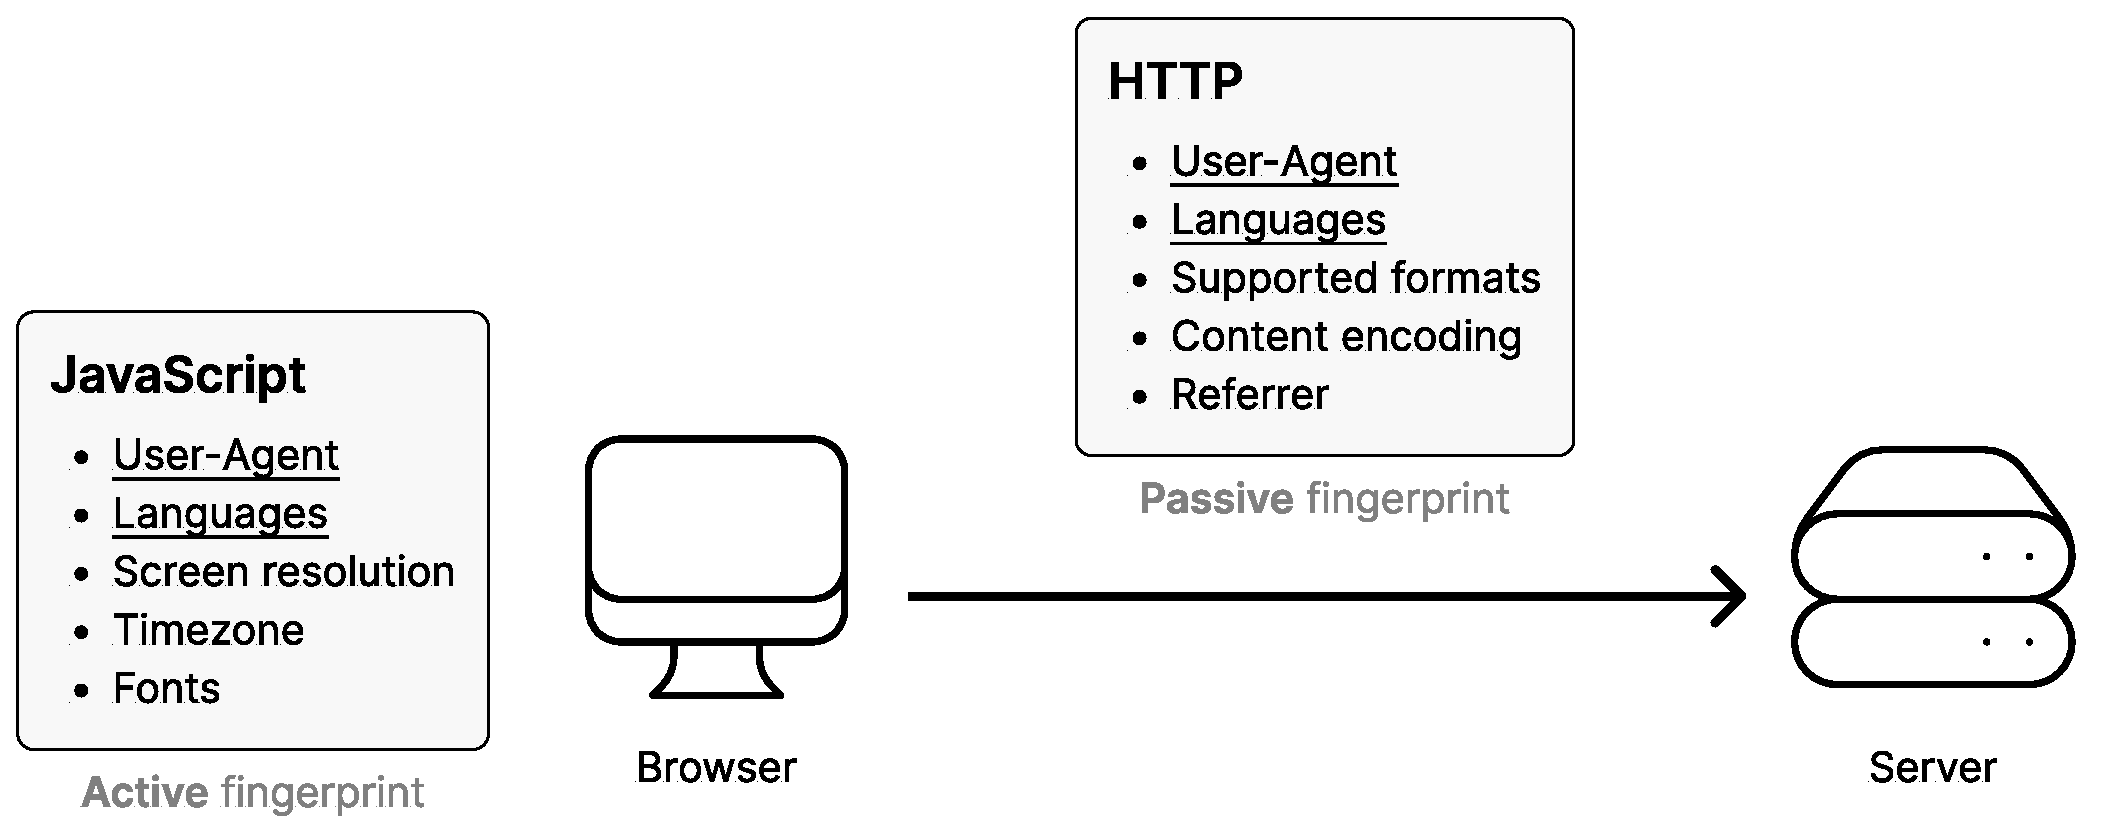
\includegraphics[width=\textwidth]{obrazky-figures/inconsistencies_schema}
    \caption{A scheme highlighting common properties obtainable with active and passive fingerprinting.}
    \label{fig:mesh1}
\end{figure}

Among the examples shown in tables \ref{Table:ActiveDataExamples} and \ref{Table:PassiveDataExamples} are characteristics with multiple data sources, namely the available memory, preferred languages, and the User-Agent string. Values of specific characteristics, such as the available memory or the User-Agent string, are one-to-one copies meaning the countermeasure algorithm can apply the same transformation to all data sources. However, this is not the case for the values of preferred languages characteristic. Preferred languages transferred in HTTP headers include the quality factor\footnote{Quality weights or quality values are used in HTTP headers to specify the order of priority in a comma-separated list (\url{https://developer.mozilla.org/en-US/docs/Glossary/Quality_values}).} for each language tag, but this value is absent in the version obtainable from the browser Web API. Tables Tables \ref{Table:ActiveDataExamples} and \ref{Table:PassiveDataExamples} illustrate this difference. An algorithm cannot apply the same transformation for all data sources as it has to be aware of these differences in representation.

Suppose a countermeasure algorithm misapplies the transformation to a data source, or the data source is left unchanged entirely. In that case, the fingerprinting application can detect and act on this attempt at fingerprint manipulation.

\section{Existing anti-fingerprinting software}

In response to the growing concerns discussed in section \ref{UnderstandingFingerprinting}, numerous anti-fingerprinting software solutions have been developed to mitigate this threat. With a focus on web-based applications, these solutions can be integrated directly into browsers or installed as browser extensions.

This section outlines selected existing anti-fingerprinting software solutions, examining their strengths and weaknesses. The primary focus has been given to the JShelter extension, which initially, this theses extended.

\subsection{Tor browser}

Tor\footnote{\url{https://www.torproject.org/}}, built on top of Mozilla Firefox, is specially designed for privacy and anonymity. Among other protections, it incorporates a variety of anti-fingerprinting measures, including:

\begin{itemize}
	\item First-party isolation to prevent cross-site tracking.
	\item Disabling or restricting access to browser features commonly used in fingerprinting, such as WebGL and WebRTC.
	\item Spoofing the user agent string to make all Tor Browser users appear identical.
	\item Enforcing a standard window size to prevent screen size-based fingerprinting.
\end{itemize}

These countermeasures are sometimes extraordinarily strict and limiting, which is precisely why they are very effective.

\subsection{Brave browser}

Brave\footnote{\url{https://brave.com/}} is another privacy-focused browser, this time based on the Chromium project. It includes several built-in fingerprinting protection mechanisms:

\begin{itemize}
	\item Blocking third-party cookies and tracking scripts.
	\item Limiting access to browser features often used for fingerprinting, such as battery status and device sensors.
	\item Randomizing specific browser characteristics, like the Canvas API or available fonts, to make fingerprinting more challenging.
\end{itemize}

Brave protections are less severe than Tor's, making Brave users less restricted but, at the same time, more prone to fingerprinting or other privacy-invading techniques.

\subsection{JShelter}

In 2019, Martin Timko designed and implemented a proof of concept browser extension called \uv{Javascript Restricter} as a part of his master's thesis \cite{MatejTimkoDP}. Inspired by his work, Libor Polčák et al. \cite{JShelterPaper} created JShelter, a browser extension focused on fingerprinting prevention, limitations of rich web APIs, prevention of attacks connected to timing, and learning information about the device, the browser, the user, and surrounding physical environment and location. JShelter offers versions for three major browsers - Firefox, Chrome, and Opera.

\subsubsection{JavaScript Shield}

The pivotal protection feature of JShelter is the JavaScript Shield \cite{JShelterJavaScriptShield}, which modifies the behavior of the JavaScript environment of the browser. JShelter provides fake information to confuse fingerprinters and make webpage-triggered attacks harder or impossible.

The JavaScript Shield internally consists of small independent pieces of code called wrappers, which modify the original behavior of JavaScript APIs available in the browser. The behavior of wrappers can be categorized followingly \cite{JShelterJavaScriptShield}:

\begin{itemize}
	\item \textbf{Precision reduction}: The original value is unnecessarily precise for most use cases. JavaScript Shield modifies the values so that typical and essential use cases are unaffected.
	\item \textbf{Providing fake information}: Some wrappers provide fake information mostly to confuse fingerprinters. For example, canvas wrappers modify the image so that the exact instructions produce a different result in each session and for each domain.
	\item \textbf{Hiding information}: JavaScript Shield hides information from selected browser APIs that are generally unnecessary or have little use. Depending on the API, it might return an error, an empty value, or block the API completely.
\end{itemize}

To modify the values of the browser characteristics, the JavaScript Shield uses a technique called \emph{farbling} \cite{JShelterPaper}. This technique is based on the implementation of farbling in Brave \cite{BraveFingerprintingDefences2}, which has its roots in previous privacy research, including the PriVaricator \cite{PriVaricator} and FPRandom \cite{FPRandom}.

Farbling first deterministically generates a per-session, per-eTLD+1\footnote{eTLD+1 is a part of a domain name, including TLD, eTLD and one more domain part (More on \url{https://jfhr.me/what-is-an-etld-+-1/}).} seed. This seed is later used to slightly randomize the output of web APIs typically used for fingerprinting. The way a seed is generated makes cross-site and cross-session tracking difficult for fingerprinting applications.

% -------------------------------------------------------------------- %

\chapter{Design proposal}
\label{Chapter:Design}

% TODO: Update the introduction

This work aims to design and implement a new protective shield for the JShelter extension that can misrepresent information commonly used for passive fingerprinting. The first section of this chapter emphasizes the importance of avoiding alterations that could disrupt the user experience. Each of the following sections describes a selected HTTP header, proposes a modification to its value, the advantages and disadvantages of this modification, and necessary changes to the browser APIs to maintain consistency.

\section{Minimizing undesired side effects}

Whenever a user loads a webpage, the browser is responsible for constructing the outgoing HTTP request. Headers included in these requests provide valuable additional information servers use to decide on the response. By default, browsers set the headers according to their best knowledge to maximize speed and compatibility.

Protections that modify header values have to do so carefully. No matter how small the change is, it can affect the server's response. For example, English is the prevalent language used on the web. To make the fingerprint look more homogenous, the protection could modify the \texttt{Accept-Language} header to report English as the preferred language. However, the user may need help understanding the content if the server reacts and actually returns a website in English.

On the other hand, the alterations made to header values should be substantial enough to obfuscate the device's fingerprint effectively. Striking the right balance is essential in ensuring the implemented protections can prevent fingerprinters from tracking the device while avoiding unintended consequences or errors. Each protection is designed to prevent such unintentional errors while keeping the capability to confuse fingerprinters.

\section{Fingerprinting protections}

The browser extension comprises several independent modules, each implementing passive fingerprinting protection for a single HTTP header or a group of HTTP headers. This separation of concerns allows users to enable only some protections while keeping others disabled.

\subsection{HTTP header: Accept}
\label{SectionHTTPHeaderAccept}

The \texttt{Accept} request HTTP header indicates which content types the client can understand, expressed as MIME types \cite{MDN}. It is possible to add or remove MIME types to affect the fingerprint. However, the server may react to this modification and respond with an unexpected and incompatible response body.

\bigbreak

\begin{lstlisting}[caption={An example of Accept header contents \cite{MDN}.}]
Accept: text/html, application/xhtml+xml, application/xml;q=0.9, image/webp, */*;q=0.8
\end{lstlisting}

\medbreak

The protection algorithm removes certain MIME types, which do not result in incompatibility, but only a slight performance hit. For example, eliminating modern image formats such as \texttt{image/webp} and forcing the browser to use older image formats is possible. This transformation would affect the header value (and, transitively, the device's fingerprint) without potentially breaking the website.

\subsubsection{Consistency}

Browsers no longer offer a standard API for quickly checking supported MIME types. The \texttt{Navigator.mimeTypes} API that partially allows this check has been deprecated and removed from the relevant web standards \cite{MDNNavigatorInterface}. A fingerprinting application could maintain a list of browser versions and supported MIME types which it would use to compare with the MIME types in the \texttt{Accept} HTTP 

Maintaining consistency but also checking the consistency is not trivial when it comes to the supported MIME types. Therefore, no browser API modifications are necessary.

\subsection{Accept-Language}
\label{SubSection:AcceptLanguage}

The \texttt{Accept-Language} request HTTP header indicates the natural language and locale that the client prefers \cite{MDN}. It is a list of language tags separated by commas (\uv{,}). A language tag consists of a 2-3 letter base tag that identifies the language, optionally followed by a dash (\uv{-}) and a subtag, usually specifying the country or the region where the language is used. Language tags can optionally have a quality value (weight) represented by a decimal number separated from the tag by a semicolon (\uv{;}).

\bigbreak

\begin{lstlisting}[caption={An example of Accept-Language header contents \cite{MDN}.}, label={AcceptLanguageExample}]
Accept-Language: fr-CH, fr;q=0.9, en;q=0.8, de;q=0.7, *;q=0.5
\end{lstlisting}

\medbreak

Modifying the \texttt{Accept-Language} header is not straightforward because the web server might respond with content in a different language than the user requested. The protection only makes minor changes and works in two modes:

\begin{itemize}
	\item \textbf{Generalization}: Language regions (subtags) are removed, and only the base language tags are kept unchanged. Listing \ref{AcceptLanguageGeneralization} shows the result of generalization for the \texttt{Accept-Language} header in listing \ref{AcceptLanguageExample}. The algorithm also deduplicates language tags and updates quality values after it removes the language regions.
	\item \textbf{Randomization}: Language regions (subtags) are changed for multiregional languages like English or Spanish. Listing \ref{AcceptLanguageRandomization} shows the randomization result for the \texttt{Accept-Language} header in listing \ref{AcceptLanguageExample}.
\end{itemize}

The reasoning behind these transformations is that the difference between language forms is usually manageable for the users. For example, changing \uv{en-US} (United States English) to \uv{en-GB} (Great Britain English) might get noticed by users, but they would still understand the content.

\bigbreak

\begin{lstlisting}[caption={The result of the \uv{generalization} mode transformation of listing \ref{AcceptLanguageExample}.}, label={AcceptLanguageGeneralization}]
Accept-Language: fr, en;q=0.9, de;q=0.8, *;q=0.5
\end{lstlisting}

\begin{lstlisting}[caption={The result of the \uv{randomization} mode transformation of listing \ref{AcceptLanguageExample}.}, label={AcceptLanguageRandomization}]
Accept-Language: fr-BE, fr;q=0.9, en;q=0.8, de;q=0.7, *;q=0.5
\end{lstlisting}


\subsubsection{Consistency}

The client-preferred languages are also available through the \texttt{Navigator} interface under the \texttt{Navigator.languages} property. The languages are ordered the same way as in the \texttt{Accept-Language} header but without the quality value (weight). The first language in \texttt{Navigator.languages} is also extracted to the \texttt{Navigator.language} property. Any change to the \texttt{Accept-Language} HTTP header must be reflected in these two properties of the \texttt{Navigator} interface.

\subsection{Device-Memory}
\label{SubSection:DeviceMemory}

The \texttt{Device-Memory} request header indicates the approximate amount of available RAM on the client device. The possible values this header can carry are \verb|0.25|, \verb|0|, \verb|5|, \verb|1|, \verb|2|, \verb|4|, and \verb|8| \cite{MDN}. A preview of this header is displayed in Figure \ref{Fig:DeviceMemoryExample}. Even though this header is still experimental, it is already implemented by the Chrome browser.

\bigbreak

\begin{lstlisting}[caption={An example of Device-Memory header contents \cite{MDN}.}, label={Fig:DeviceMemoryExample}]
Device-Memory: 1
\end{lstlisting}

\medbreak

% TODO: Explain that the server has to request these headers.

The protection algorithm randomly picks one of the possible values and uses it as the value of the \texttt{Device-Memory} header.

\subsubsection{Consistency}

The value of the \texttt{Device-Memory} header is also accessible through the \texttt{Navigator.deviceMemory} property. Any transformation to the \texttt{Device-Memory} header must be copied to this property.

\subsection{User-Agent and client hints}

The \texttt{User-Agent} request HTTP header is a string that lets servers and network peers identify the application, operating system, vendor, and version of the requesting user agent \cite{MDN}. The value of this header varies depending on the operating system and browser type and version, making it a valuable fingerprint component.

\bigbreak

\begin{lstlisting}[caption={An example of Chrome User-Agent string \cite{MDNHeaderUserAgent}.}, label={Listing:UserAgentChrome}]
Mozilla/5.0 (X11; Linux x86_64) AppleWebKit/537.36 (KHTML, like Gecko) Chrome/51.0.2704.103 Safari/537.36
\end{lstlisting}

\begin{lstlisting}[caption={An example of Safari User-Agent string (mobile version) \cite{MDNHeaderUserAgent}.}, label={Listing:UserAgentSafari}]
Mozilla/5.0 (iPhone; CPU iPhone OS 13_5_1 like Mac OS X) AppleWebKit/605.1.15 (KHTML, like Gecko) Version/13.1.1 Mobile/15E148 Safari/604.1
\end{lstlisting}

\medbreak

Figures \ref{Listing:UserAgentChrome} and \ref{Listing:UserAgentSafari} show examples of \texttt{User-Agent} strings of Chrome and Safari, which according to Statcounter GlobalStats\footnote{Statcounter GlobalStats collects statistics from more than 1.5 million sites with yearly views ranging from 5 to 6 billion. These statistics are available at \url{https://gs.statcounter.com/}.}, are the top two browsers with the highest market share of 64.62\% and 18.29\%, respectively. These examples indicate that some browsers and operating systems have version numbers following the semantic versioning specification\cite{SemVerWebsite} or its variation. Semantic versioning in the most recent version 2 is composed of three segments separated by a dot (\uv{"."}), where:

\begin{itemize}
	\item The first segment (\textbf{MAJOR}) is incremented when an incompatibility, such as a breaking API change, is introduced.
	\item The second segment (\textbf{MINOR}) is incremented when new functionality is added while maintaining backward compatibility.
	\item The last segment (\textbf{PATCH}) is incremented for all other changes, for example, a bug fix or code refactoring.
\end{itemize}

Based on the observation that some software versions in the \texttt{User-Agent} string follow the semantic versioning specification, we can assume that:

\begin{enumerate}
	\item Given two version numbers differ only in the last segment (\textbf{PATCH}), we know these software builds should have the same functionalities, meaning they should be indistinguishable for the user.
	\item A change (either an increment or a decrement) of the (\textbf{PATCH}) segment value would likely affect the device's fingerprint. However, at the same time, it is unlikely that the change would cause any undesired side effects.
\end{enumerate}

The protection cannot apply changes at random, as this could introduce invalid version numbers that have yet to be released. Invalid version numbers could be used by the fingerprinting application to discover an attempt at fingerprint manipulation. Instead, the extension keeps a list of previously released versions gathered from the changelog\footnote{Software products typically maintain a list of published versions. For example, the changelog of Chrome is available at \url{https://chromereleases.googleblog.com/search/label/Stable\%20updates.]}} of the specific software product. The algorithm then randomly selects a suitable version that only differs in the \textbf{PATCH} segment and should have the same functionality as the original version.

\bigbreak

\begin{lstlisting}[caption={An example of HTTP Client hints \cite{MDN}.}, label={Listing:HTTPClientHintsExample}]
Sec-CH-UA: " Not A;Brand";v="99", "Chromium";v="96", "Google Chrome";v="96"
Sec-CH-UA-Mobile: ?0
Sec-CH-UA-Full-Version: "96.0.4664.110"
Sec-CH-UA-Platform: "Windows"
\end{lstlisting}

\medbreak

The \texttt{User-Agent} is not the only HTTP header from which the fingerprinter can gain detailed information about the device's browser and platform. The same information can also be extracted from HTTP Client hints. Client Hints are a set of HTTP headers that enable websites to request and receive specific information about a user's device and preferences directly from the browser \cite{MDN}. Client Hints can be broadly classified into two categories based on their entropy levels:

\begin{itemize}
	\item \textbf{Low entropy client hints}: These headers provide limited variability and do not significantly contribute to unique browser fingerprints. Examples of low entropy headers include \texttt{Save-Data}, \texttt{Viewport-Width}, and \texttt{DPR} (Device Pixel Ratio). These headers usually pose a low risk to user privacy.
	\item \textbf{High entropy client hints}: These headers provide a higher level of variability and may be used to create more accurate browser fingerprints, posing a higher risk to user privacy. Examples of high entropy headers include \texttt{Sec-CH-UA} (\texttt{User-Agent}), \texttt{Sec-CH-UA-Platform-Version}, and \texttt{Sec-CH-UA-Full-Version} (full browser version).
\end{itemize}

From the fingerprinting point of view, the high entropy values are more important because they tend to change less often, if ever. The extension modifies selected client hints carrying the characteristics which can also be found in the \texttt{User-Agent} header. This additional layer ensures consistency across all HTTP headers and better protection against fingerprinting.

\subsubsection{Consistency}

The \texttt{User-Agent} string can also be accessed through the JavaScript \texttt{Navigator} interface. This value is identical to the one transmitted in the \texttt{User-Agent} HTTP header when a client makes a request to a web server. To maintain consistency between the two sources of the \texttt{User-Agent} string, applying the same transformation or parsing logic to the value obtained from \texttt{Navigator.userAgent} is crucial. This consistency ensures that the information is treated uniformly and helps to prevent a potential discovery by comparing the strings.

\bigbreak

\begin{lstlisting}[caption={An example the User-Agent Client Hints API usage \cite{MDN}. This API call returns the same values as the HTTP client hints in example \ref{Listing:HTTPClientHintsExample}.}]
navigator.userAgentData
  .getHighEntropyValues([
  	"mobile"
    "platform",
    "uaFullVersion",
  ])
  .then((ua) => {
    console.log(ua);
  });	
\end{lstlisting}

\medbreak

To also ensure the HTTP client hints are consistent with the browser environment, the extension must modify the return values of the \texttt{navigator.userAgentData}\footnote{\url{https://developer.mozilla.org/en-US/docs/Web/API/User-Agent_Client_Hints_API}} API. Although this API is still marked as experimental, it is already supported by Chromium-based browsers. In fact, the only major browser which doesn't support this API is Firefox.

\subsection{Extra HTTP header}
\label{SubSection:ExtraHTTPHeader}

One of the valuable characteristics used to construct a fingerprint is the list of all headers present in a request. Most requests share standard headers like those mentioned in previous sections X, Y, and Z. However, it is common for HTTP requests to include less standard, even custom\footnote{Until 2012, developers tended to prefix custom headers with \uv{X-} to differentiate them from standardized headers, but this naming convention has been officially discouraged in RFC6648 \cite{RFC6648}.} headers.

\bigbreak

\begin{lstlisting}[caption={An example of a list of headers present in an HTTP request.}]
Accept, Accept-Encoding, Accept-Language, Connection, Cookie, Host, User-Agent
\end{lstlisting}

\medbreak

The protection adds a new header to the HTTP request to alter the list and order of headers and transitively the device's fingerprint. Additionally, if the newly added header is custom and not standardized by the protocol, this change would likely not affect the response.

\section{Graphical user interface}
\label{Section:GUI}

The popup is the only graphical user interface the extension exposes. This view contains preferences users can use to change the behavior of the fingerprinting protections.

\medbreak

\begin{figure}[H]
\centering
\begin{subfigure}{.5\textwidth}
  \centering
  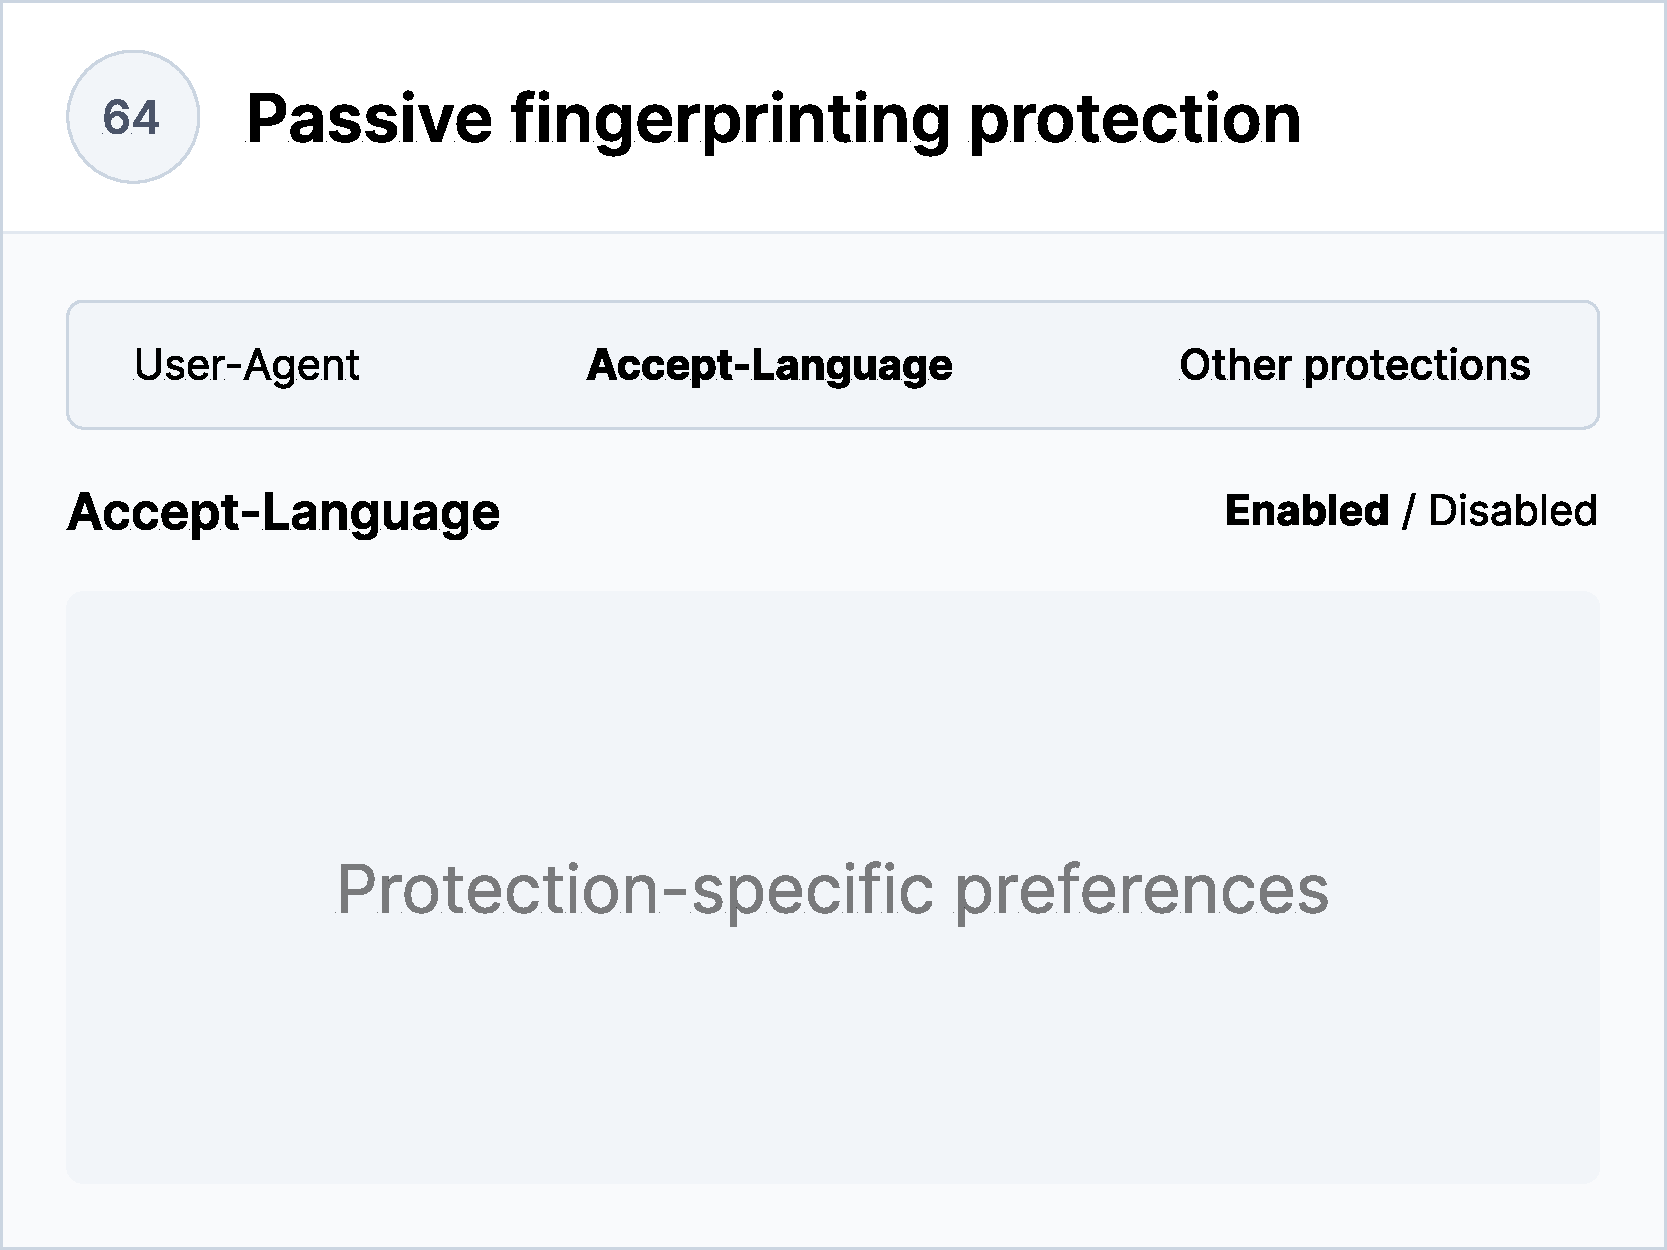
\includegraphics[width=.95\linewidth]{obrazky-figures/wireframe}
  \caption{Light mode wireframe.}
\end{subfigure}%
\begin{subfigure}{.5\textwidth}
  \centering
  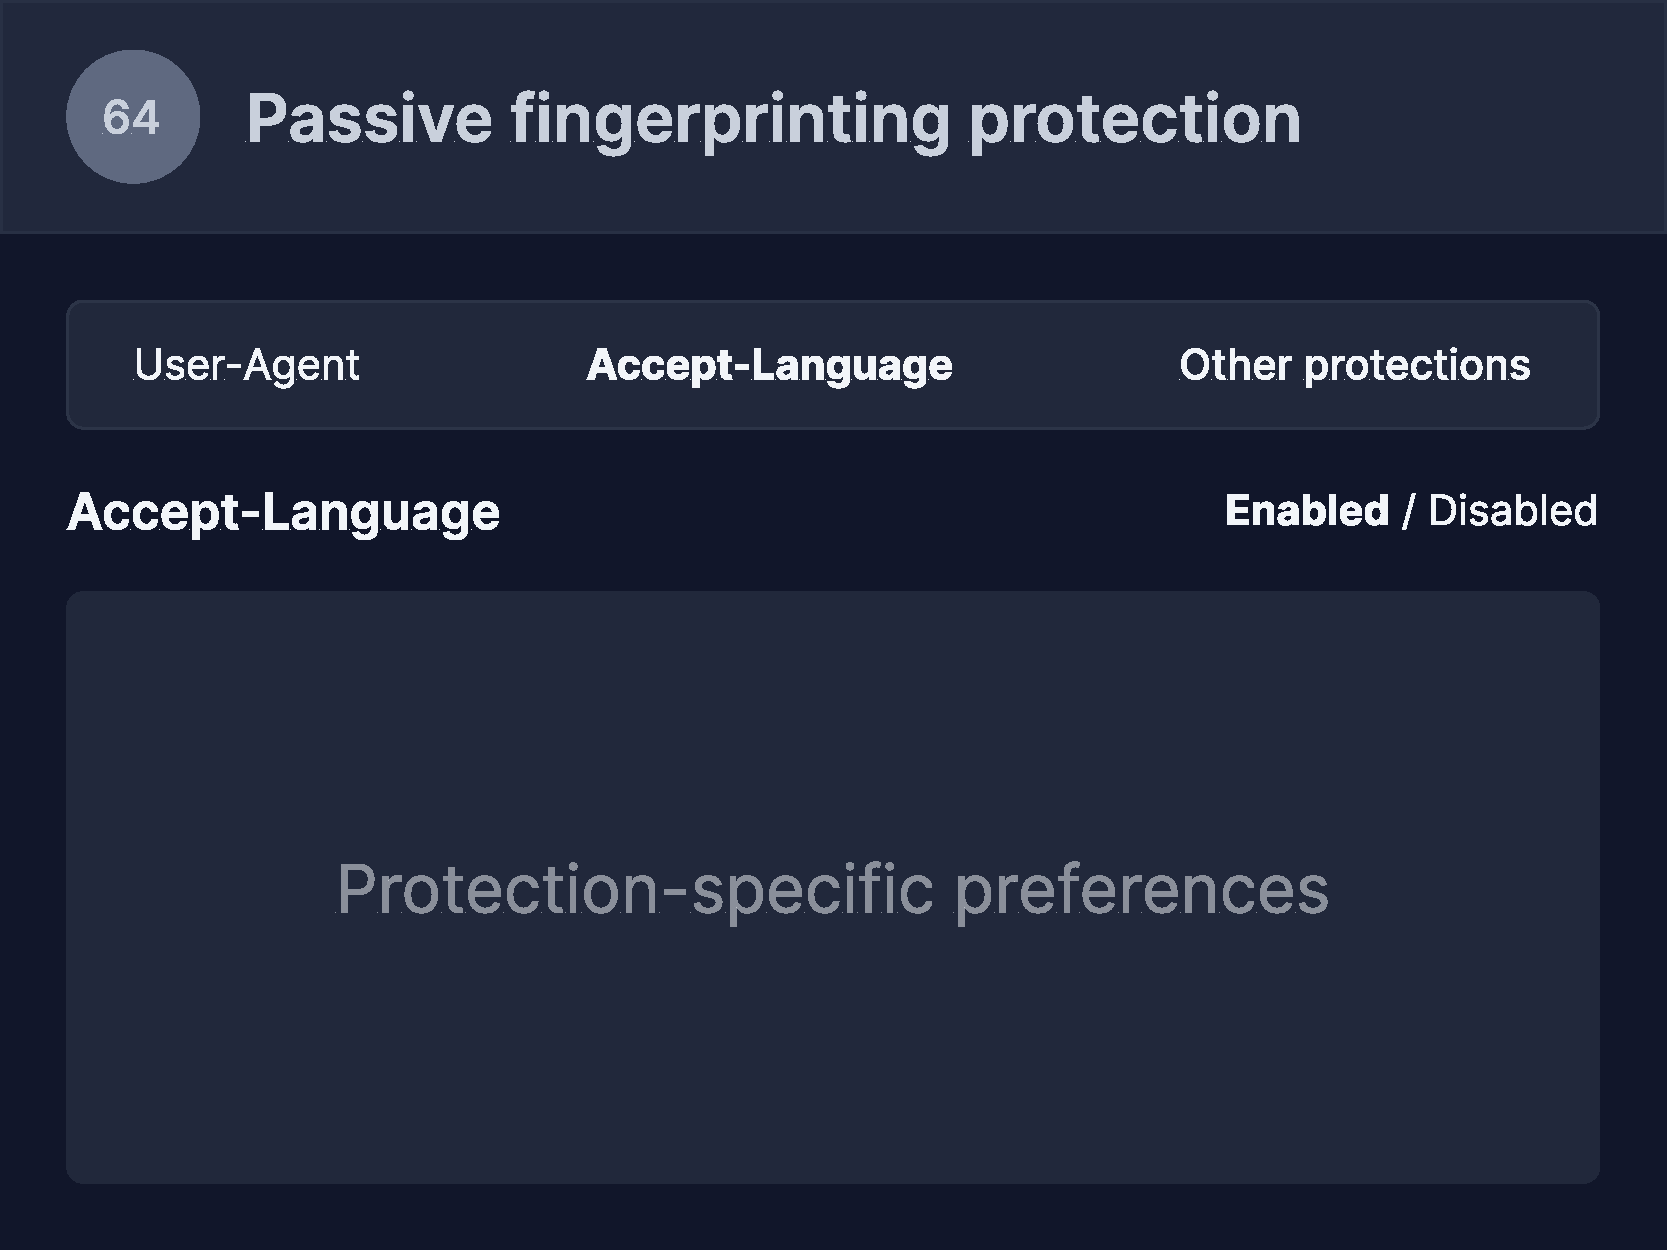
\includegraphics[width=.95\linewidth]{obrazky-figures/wireframe-dark}
  \caption{Dark mode wireframe}
\end{subfigure}
\caption{A comparison of light and dark mode wireframes of the browser extension.}
\label{Fig:Wireframes}
\end{figure}

\medbreak

The preferences are split into three tabs (views). This division allows for more prominent controls and descriptive hints that help users understand what each option does. The first two tabs contain preferences for the most influential HTTP headers, \texttt{User-Agent} and \texttt{Accept-Language}. The last tab groups other, less significant protections, such as \texttt{Device-Memory}.

Each protection can be enabled or disabled individually from others. When enabled, a preview field will appear under the protection's preferences. The preview field shows the header value as it will be sent in future outgoing requests and is updated automatically according to the selected preferences.

Modern operating systems have to option to switch the user interface to a dark mode which complements the standard light color scheme. The extension's popup view and every component it renders are made in light and dark variants. The extension automatically switches between these variants based on the operating system's active color scheme. Figure \ref{Fig:Wireframes} displays browser extension wireframes in both light and dark modes.

\chapter{Implementation}

% TODO: Update the introduction

\section{Development environment and tools}

This section discusses the programming languages, libraries, frameworks, and other tools used to develop the browser extension. The rationale behind choosing these technologies and how they contribute to the effectiveness of the extension is also explained.

\subsection{TypeScript}

TypeScript\footnote{\url{https://www.typescriptlang.org/}}, a statically typed superset of JavaScript, was chosen as the primary programming language. TypeScript provides type safety, which helps catch errors during development and makes the codebase easier to maintain and refactor. Moreover, TypeScript's advanced type features improve code readability and provide better support for modern IDEs, enhancing the development experience.

\subsection{React}

React\footnote{\url{https://react.dev/}}, a popular JavaScript library for building user interfaces, was employed for creating the extension's UI components. React's component-based architecture promotes modularity and reusability, simplifying the development process and ensuring maintainable code. Furthermore, React's virtual DOM enhances the performance of the browser extension by reducing the need for frequent DOM manipulations, which can be resource-intensive.

\subsection{Radix UI}

Radix UI\footnote{\url{https://www.radix-ui.com/}}, a set of low-level, unstyled, accessible, and composable UI components for React, was integrated into the project to streamline the browser extension's UI development. Using Radix UI components ensures that the extension's UI adheres to accessibility best practices and provides a solid foundation for customization. Thanks to its focus on accessibility, Radix UI offers a consistent user experience across different platforms and devices.

\subsection{Tailwind CSS}

Tailwind CSS\footnote{\url{https://tailwindcss.com/}}, a utility-first CSS framework, was utilized to style the browser extension's user interface. Tailwind CSS enables rapid UI development by providing predefined CSS utility classes, which can be easily combined to create custom styles. This approach reduces the need for writing custom CSS, leading to a more streamlined development process and a consistent design language across the extension. Although Tailwind CSS offers a wide variety of utility functions, only the ones used by the extension make it to the final bundle, keeping the size low.

\subsection{Vite}

Vite\footnote{\url{https://vitejs.dev/}}, a modern build tool and development server, was selected to handle the project's build process and improve the development experience. Vite offers fast development server startup and on-demand compilation, resulting in a more efficient and productive development environment. Additionally, Vite supports various output formats, making integrating the browser extension into different browsers easier. 
	
The \texttt{vite-plugin-web-extension}\footnote{\url{https://github.com/samrum/vite-plugin-web-extension}} installed on top of Vite allows for easier creation of cross-browser extensions with support for ES Modules and HMR\footnote{\url{https://webpack.js.org/concepts/hot-module-replacement/}}.

\section{Browser extension components}

This section provides a detailed breakdown of the main components that make up the browser extension, explaining their functionality and how they interact with one another.

\subsection{Storage and data management}

The extension uses the \texttt{storage} API to store and persist user settings and extension state. This API bears similarities to the conventional Web Storage API\footnote{\url{https://developer.mozilla.org/en-US/docs/Web/API/Web_Storage_API}}, with an important distinction being that its scope is not bounded to a domain but is instead associated with the extension itself. In particular, the extension stores its data in the \texttt{storage.sync}\footnote{\url{https://developer.mozilla.org/en-US/docs/Mozilla/Add-ons/WebExtensions/API/storage/sync}} storage area, automatically synchronizing with all browser instances where the user is signed in.

Each passive fingerprinting protection stores its preferences in a separate part of the storage space. In addition to the protection-specific settings, each protection shares two common fields:

\begin{itemize}
	\item \textbf{enabled}: A boolean flag determining if the protection is enabled, meaning the browser extension should enable the rule responsible for changing the value of a specific HTTP header.
	\item \textbf{value}: A string representing the current value of the HTTP header, incorporating all protection-specific preferences. It is displayed in the popup interface to provide the user with a preview of the particular HTTP header.
\end{itemize}

The storage is the centerpiece of the browser extension. Other components, including the service worker and user interface, rely on the storage to synchronize their actions, given that they execute in separate contexts.

\subsection{Service worker}

% TODO: Content

\subsection{User interface}

As section \ref{Section:GUI} describes, the popup is the only graphical user interface used by the browser extension. The popup consists of one HTML file, which does not directly render UI elements. Instead, it initializes a React application which takes over the rendering. By delegating the rendering process to the React application, the popup benefits from React's dynamic and efficient nature, allowing for enhanced performance, maintainability, and ease of development when managing the extension's user interface.

\bigbreak

\begin{lstlisting}[caption={A code snippet in which the React application initializes its storage and creates a subscription for future changes.}]
useEffect(() => {
  if (typeof unsubscribe.current === 'function') {
    unsubscribe.current();
  }

  void browser.storage.sync.get().then((store: StoreValue | {}) => {
    if (isStoreInitialized(store)) {
      initializeStore(store);
    }

    unsubscribe.current = useStore.subscribe((store) => {
      void browser.storage.sync.set(store);
    });
  });
}, []);
\end{lstlisting}

\medbreak

Immediately after the initialization, the React application connects to the extension's storage, copies the content to its internal data storage, and subscribes for future changes. Utilizing an internal storage layer between the application and the browser storage was essential due to the asynchronous nature of the browser storage. If every read or write operation was performed directly on the browser storage, the UI would only be allowed to update once the operation was completed, resulting in a sluggish user experience. The application can mitigate this issue by utilizing an internal storage layer, ensuring a more responsive and seamless interface. Every change to the internal storage is automatically synchronized with the browser storage.

\bigbreak

\begin{lstlisting}[caption={A part of the code that updates the HTTP header-modifying rule when a protection is enabled or disabled.}]
useEffect(() => {
  if (enabled && value !== null) {
    updateHeaderRule(Header.ACCEPT_LANGUAGE, value);
  } else {
    removeHeaderRule(Header.ACCEPT_LANGUAGE);
  }
}, [value, enabled]);
\end{lstlisting}

\medbreak

The popup interface is separated into multiple sections exclusive to specific protections. Each protection section has a header, a switch to enable or disable the protection, and a preview field with the current header value. If protection has custom preferences, these are also colocated with these primary elements. Whenever a user changes protection-specific preferences, the extension automatically updates the \texttt{value} field in storage, which propagates to the UI. However, the rule modifying the header value is only updated when the protection is enabled or disabled.

\section{Fingerprinting protections}

This section describes the browser extension's specific strategies to combat passive fingerprinting through HTTP headers. Each method is discussed in detail, accompanied by relevant implementation examples. Furthermore, any deviations from the initial design plan are highlighted and explained throughout this section.

\bigbreak

\begin{lstlisting}[caption={A utility function that removes the old header-modification rule and defines a new one with a new value.}, label={Listing:UpdateRuleFunction}]
export const updateHeaderRule = (header: Header, value: string) => {
  const id = HEADER_RULE_IDS[header];

  void browser.declarativeNetRequest.updateSessionRules({
    removeRuleIds: [id],
    addRules: [
      {
        id,
        priority: 1,
        action: {
          type: 'modifyHeaders',
          requestHeaders: [
            {
              header: header,
              operation: 'set',
              value,
            },
          ],
        },
        condition: {
          urlFilter: '*://*/*',
          resourceTypes: ['main_frame'],
        },
      },
    ],
  });
};

\end{lstlisting}

\medbreak

In order to effectively manage the header-modification rules, a unique identifier is assigned to each HTTP header, serving as the rule's ID that does not change for the complete run of the extension. Whenever a rule needs to be updated, protections call a utility function (shown in listing \ref{Listing:UpdateRuleFunction}) with two arguments - the header's name and its new value.

\subsection{User-Agent and client hints}

% TODO: Content

\subsection{Accept-Language}

As section \ref{SubSection:AcceptLanguage} defines, the browser extension modifies the \texttt{Accept-language} header in two modes -- randomization and generalization. Both modes start by looking at the contents of \texttt{Navigator.languages} and selecting only the language codes with the ISO-639 subtag. These language codes are identified by checking if they include a dash (\uv{-}) separating the language tag from the subtag.

The randomization algorithm then checks whether one or more languages have subtag alternatives. If yes, it randomly selects a subtag from all the possible alternatives and replaces the original subtag. The algorithm can also select the original subtag to prevent the fingerprinting application from guessing it by narrowing the options.

On the other hand, the generalization algorithm removes subtags from all language codes leaving only the base language tags (i.e., \uv{en} or \uv{zh}).

Upon completion of the transformation algorithms, the main program verifies the validity of the resulting list of languages. Initially, it eliminates any duplicate values that may have been introduced by the generalization or the randomization algorithm, which could select two or more identical subtags. The generalization algorithm always introduces duplicates if the original list of languages includes the same language tag more than once (i.e., \uv{en, en-US, en-GB}).

In the final step, the algorithm takes the resulting list of languages, calculates the quality values for each language, and joins them into a single string, using a comma (\uv{,}) as the delimiter. The quality value is determined by the position of the language in the list of languages. The first language does not have a quality value as it is the primary language and has an implicit value of \texttt{1.0}. Each following language has a quality value equal to \texttt{1.0 - index * 0.1}. After this step, the resulting string is ready to be used as the value of the \texttt{Accept-Language} header.

\subsection{Device-Memory}

In its nature, the protection modifying the \texttt{Device-Memory} is very straightforward, and the rationale behind it is explained in section \ref{SubSection:DeviceMemory} of the previous chapter.

Initially, the algorithm retrieves the user-configured min and max values from the popup interface. These values represent the minimum and maximum indices within the array of permissible \texttt{Device-Memory} values, which include \texttt{0.25}, \texttt{0.5}, \texttt{1}, \texttt{2}, \texttt{4}, and \texttt{8}.

Subsequently, the algorithm randomly chooses a value between the specified min and max indices. The randomized selection introduces an element of unpredictability, making it more challenging for fingerprinters to identify the actual user's device memory accurately. Once the value is selected, the algorithm returns it as the modified \texttt{Device-Memory} header, ensuring that the user's actual device memory remains concealed.

\subsection{Extra HTTP header}

According to the design discussed in section \ref{SubSection:ExtraHTTPHeader}, this protection adds a new, non-standard header \texttt{Extra} to each outgoing request. The value of this request is determined by the native function \texttt{Crypto.randomUUID()}. This function returns a UUID, a 128-bit long value represented as a 36-character string, which is guaranteed to be unique across space and time \cite{RFC4122}.

\section{Challenges and limitations}

This section discusses the challenges encountered throughout the implementation process and the corresponding strategies to address them, where applicable.

\subsection{Manifest V3}

During the time of writing, the new Manifest V3 has begun replacing the outgoing Manifest V2. Although the official end-of-life support deadline for Manifest V2 has been postponed, the browser extension discussed in this thesis has been developed utilizing the latest Manifest V3 framework. This design decision led to a series of challenges described in the following paragraphs.

The biggest obstacle was the deprecation of the blocking web request listeners previously available through the \texttt{chrome.webRequest} API. Rather than intercepting requests and modifying them in real-time using the \texttt{chrome.webRequest} API, extensions must define request-altering rules through the \texttt{chome.declarativeNetRequest} API before the browser sends the request. Since the rules are defined beforehand, it is impossible to base the new HTTP headers on the original values sent by the browser. Instead, the extension has to use the available Web APIs to approximate the header values.

% TODO: Modification of JS APIs

Finally, Manifest V3 is a relatively recent development in browser extension frameworks. As a result, the available resources and documentation detailing its inner workings, best practices, and nuances could be more extensive.

\subsection{Chrome's User-Agent reduction}

Beginning with Chrome version 101, the browser replaced parts of the User-Agent string with static values to protect the user's privacy. Version 101\footnote{\url{https://groups.google.com/a/chromium.org/g/blink-dev/c/dcTStiBZVoQ/m/KyomPLOnAwAJ}} replaced the \textbf{MINOR}, \textbf{BUILD}, and \textbf{PATCH} version segments with zeros, only leaving the \textbf{MAJOR} segment displaying the actual version (i.e., \texttt{101.0.0.0}). Next, in version 107\footnote{\url{https://groups.google.com/a/chromium.org/g/blink-dev/c/kC-AeZ1fSdY/m/a_ICuXZRBQAJ}}, the browser replaced the desktop OS version and CPU information with a fixed value for the platform. The latest reduction happened in version 110\footnote{\url{https://groups.google.com/a/chromium.org/g/blink-dev/c/zVOEHwgyyu4/m/8KljdSN9AQAJ}}, where the browser started using a fixed OS version and device model value for Android devices.

While these changes are certainly welcomed from a privacy standpoint, these reductions prevented the implementation of the \texttt{User-Agent} modifying protection, as any change made to this header would be instantly detectable by fingerprinting applications, potentially compromising the effectiveness of the privacy protection.

% TODO: Client hints


% For compilation piecewise (see projekt.tex), it is necessary to uncomment it
% \end{document}